% Preamble
\documentclass[11pt]{article}
\usepackage{graphicx}
\usepackage[margin=1in]{geometry}

\usepackage{makeidx}  % allows for indexgeneration
\usepackage{ifpdf}
\usepackage{url}


\title{Elementary Cellular Automata as an Error Minimized Hash}
\date{November 2024}
\author{Daniel McKinley}

% Document
\begin{document}

\maketitle

\section{Introduction}

Elementary cellular automata are extensions of logic gate truth tables done linearly in parallel. \cite{Wolfram}
Here they are explored as a file hash and signal hash algorithm, minimizing discrepancies between
the input and output data by choosing the correct row 0 input neighborhood for a given 0-255 ECA rule.
Unique solutions and best performing elementary automata rules are identified, several parameters
are explored for effect on behavior, and existing literature is reviewed \cite{hashSchemes}. It is implemented in Java at \cite{mygit}. 
\\
\section{Main Algorithm}

The algorithm has 3 properties of a good hash algorithm, and 2 that make it more suitable as a
signal hash rather than a block data hash [some hash paper citation]. Each input has a unique
solution, the solutions are distributed evenly across all possible solutions, and it loses less
than half the bits per compression cycle. Small changes to the input do not produce large changes
in the solution, and errors in compression are semi uneven which is mitigated in context of a signal.
\\
\\
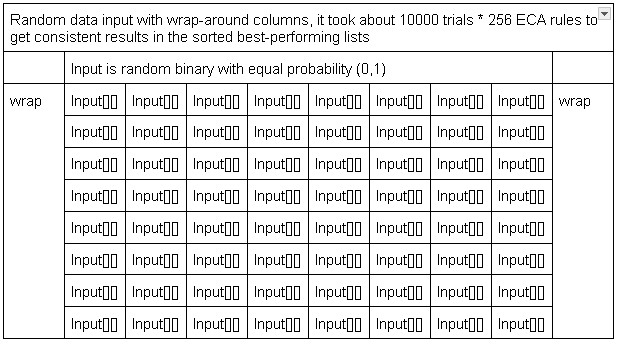
\includegraphics{WrappedInput}\\
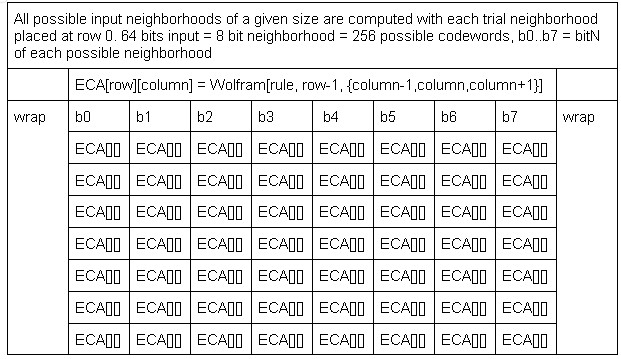
\includegraphics{ECAspace}\\
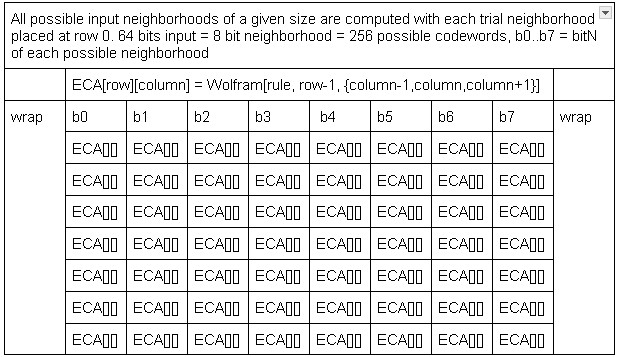
\includegraphics{ErrorScore}\\
\\
\subsection{Hash properties}

\subsubsection{Unique Minimums}
Certain ECA rules reduce to unique solutions for any given input. Another overlapping set
reduces to a unique solution when the errorScore is calculated with an exponent of 4 instead of 2.
\\
\subsubsection{Even distribution of solutions}
All possible solutions for any given rule have an equal probability of occuring over enough
iterations of random input.
\\
\subsubsection{Accuracy}
Certain ECA rules, including a large overlap with the XOR additive rules [citation] have
better than 2/3 accuracy/bit with most rules having better than 1/2 accuracy/bit over all
the input bits. The wrapped/non-wrapped tradeoff is 2/3 accuracy and an uneven errors/row w
hen done repeatedly or 1/2 accuracy and linear errors/frequency. In the non-wrapped signal
version the best performing rules had better than 1/2 accuracy/bit.
\\
\subsubsection{Error distribution}
Errors are distributed equally across columns, and with the errors in the last row roughly
half that of the first row. In the context of a signal you would have a tendency to linearly
lose more in either the high or low frequencies.
\\
\subsubsection{Distance between codewords}
If you change the input of a given (input, solution) and score the difference the same way
you score the error that gets minimized, the mean changeScore per Hamming change in the
codeword is roughly 100, corresponding to a one bit difference at any column between
row 6 and row 7 where $2^row = changeScore/bit$.
\\
\section{Post-analysis}


\subsection{Individual rules' performance}
Results are checked for all neighborhoods with stochastic input, roughly 10000 are
required for consistent results in some categories. Rules 90,60,102,153 are the best
performing rules in terms of accuracy with several class 4 rules performing almost as
well as the Pascal triangle set. When the error scoring exponent is changed to 4
instead of 2, several more members of the XOR additive rules perform well.
\\
\subsection{Class 4 rules}
Several class 4 ECA rules perform well in the hash algorithm, indicating that in
future iterations of the project some types of data and some types of noise
affect the ideal ECA hash for a given situation beyond what is presented here.
\\
\subsection{Wrapped v non-wrapped}
A non wrapped version of the calculation space is checked. The accuracy goes down and solutions become non-unique.
\\
\bibliographystyle{plain}
\bibliography{HashBib.bib}

\end{document}